\documentclass[conference]{IEEEtran}
\usepackage[utf8]{inputenc}
\usepackage[T1]{fontenc}
\usepackage{amsmath,amssymb}
\usepackage{graphicx}
\usepackage{booktabs}
\usepackage{array}
\usepackage{multirow}
\usepackage[numbers,sort&compress]{natbib}
\usepackage{hyperref}
\usepackage{xcolor}
\usepackage{enumitem}
\usepackage{caption}
\usepackage{float}
\usepackage{colortbl}
\usepackage{tabularx}
\sloppy

\definecolor{headerblue}{RGB}{30,80,160}
\definecolor{lightgray}{gray}{0.93}
\definecolor{riskred}{RGB}{200,50,50}
\definecolor{riskamber}{RGB}{200,140,0}
\definecolor{riskgreen}{RGB}{40,140,40}

\hypersetup{
  colorlinks=true,linkcolor=blue!60!black,
  citecolor=blue!60!black,urlcolor=blue!60!black,
  pdftitle={The Evolution of LLM Safety Architectures},
  pdfauthor={Simarjot Singh Maan}
}

\begin{document}

\title{SENTINEL: Semantic Evaluation, Network Trajectory Integrity, and Node-based Enforcement Logic}

\author{%
  \IEEEauthorblockN{Simarjot Singh Maan}
  \IEEEauthorblockA{Independent AI Safety Researcher\\
  \texttt{simarjotsinghmaan@gmail.com}}
}

\maketitle

\begin{abstract}
Standard LLM safety mechanisms -- keyword filtering and behavioral
alignment~\cite{ouyang2022training,bai2022constitutional} -- fail under
adversarial conditions documented across major
benchmarks~\cite{wei2023jailbroken,zou2023universal,mazeika2024harmbench,
chao2024jailbreakbench}.
This paper makes four contributions.
First, a five-phase Systemization of Knowledge (SoK) taxonomy of LLM safety
architectures, each phase analyzed by enforcement locus, threat model, and
residual failure mode.
Second, a nine-layer Safety Alignment Pipeline (SAP) framework distributing
enforcement responsibility across preprocessing, training, inference, and
orchestration tiers.
Third, an Ideal Anti-Jailbreak Defense Architecture (IAJDA) whose eight layers
each target a specific mechanistic failure mode identified in the SoK.
Fourth -- and most centrally -- empirical validation of SENTINEL, a
five-layer prototype implementation of IAJDA, evaluated against four
open-weight models ($\leq$9B parameters): Meta Llama~3.1~8B, Qwen~2.5~7B,
Gemma~2~9B, and Mistral~7B-Instruct~v0.3.
Across 500$+$ adversarial prompts tested across all models, drawn from JailbreakBench,
HarmBench, and HH-RLHF~\cite{chao2024jailbreakbench,mazeika2024harmbench,bai2022training},
SENTINEL achieves 100\% block rate on direct harmful, context manipulation,
prompt injection, prompt leakage, multi-step escalation, and agent delegation
categories, 96\% on roleplay/persona attacks, and 88\% on encoded/obfuscated
inputs -- compared to average baseline block rates of 46\%, 4\%, 65\%, 38\%,
25\%, and 33\% respectively.
Zero false positives were observed across 30 benign control prompts.
Observed latency (3.4--92\,s on an RTX~4050) reflects local compute bottlenecks;
production GPU infrastructure is expected to reduce end-to-end latency by
$\sim$10$\times$, approaching $\leq$1\,s.
\end{abstract}

\begin{IEEEkeywords}
LLM safety, jailbreak defense, adversarial robustness, alignment pipeline,
SENTINEL prototype, empirical evaluation, prompt injection, attack taxonomy
\end{IEEEkeywords}

% ======================================================
\section{Introduction}
\label{sec:intro}

Early LLM safety treated harmful outputs as a filtering problem.
Keyword blocklists failed quickly: character substitution, misspelling, and
indirect phrasing preserved adversarial intent while evading surface-form
checks.
Reinforcement Learning from Human Feedback
(RLHF)~\cite{ouyang2022training,christiano2017deep} improved matters
substantially but did not close the gap.
HarmBench~\cite{mazeika2024harmbench} results confirm that RLHF-aligned models
sustain non-trivial Attack Success Rates (ASR) under gradient-based suffix
attacks~\cite{zou2023universal}, encoding bypass~\cite{chu2024comprehensive},
and persona-substitution
jailbreaks~\cite{wei2023jailbroken}.
Our own experiments, reported here for the first time, confirm these patterns
persist across all four evaluated open-weight models under eight distinct attack
categories.

This paper provides a unified SoK account of how safety enforcement has
evolved across five phases and introduces SENTINEL -- a fully implemented,
empirically validated five-layer defense prototype demonstrating that
substantial safety improvement is achievable without changes to model weights.
Our contributions are as follows.
\begin{enumerate}[leftmargin=1.4em,itemsep=1pt]
  \item A five-phase SoK taxonomy of LLM safety architectures organized by
    enforcement locus and failure mode (Section~\ref{sec:taxonomy}).
  \item A nine-layer Systemic Alignment Pipeline (SAP) framework
    (Section~\ref{sec:sap}).
  \item A mechanistic account of eight persistent attack families with
    benchmark-grounded ASR values (Section~\ref{sec:jailbreak}).
  \item Empirical evaluation of SENTINEL across four open-weight models on
    500$+$ adversarial prompts and 30 benign controls
    (Section~\ref{sec:experiments}).
  \item Theoretical grounding for verbosity-based anomaly detection and
    a discussion of false-positive amplification in layered defenses
    (Sections~\ref{sec:sentinel} and~\ref{sec:discussion}).
\end{enumerate}

% ======================================================
\section{Background and Related Work}
\label{sec:background}

\textbf{RLHF and DPO.}
RLHF~\cite{christiano2017deep,ouyang2022training} fine-tunes a policy via
proximal policy optimization against a human-preference reward model with
a KL-divergence penalty.
Safety-focused RLHF variants~\cite{bai2022training} add adversarial prompt
categories but remain susceptible to reward
overoptimization~\cite{gao2023scaling} and distributional gaps.
DPO~\cite{rafailov2023direct} simplifies the pipeline to direct preference
optimization, achieving competitive alignment at lower compute, though targeted
prompting partially undermines both approaches~\cite{yang2023shadow}.

\textbf{Constitutional AI and RLAIF.}
CAI~\cite{bai2022constitutional} applies written normative principles through
self-critique before preference learning, making alignment auditable.
RLAIF~\cite{lee2023rlaif} substitutes AI feedback for human labels, improving
scalability.
Both remain vulnerable to distributional
attacks~\cite{zou2023universal,anil2024many}.

\textbf{Adversarial Benchmarks.}
JailbreakBench~\cite{chao2024jailbreakbench} provides reproducible evaluation
over 100 standardized harmful behaviors with public leaderboards.
HarmBench~\cite{mazeika2024harmbench} covers 510 behaviors across 7 functional
categories and supports automated red-teaming evaluation.
HH-RLHF~\cite{bai2022training} provides preference pairs covering both
helpfulness and harmlessness dimensions, widely used for alignment training and
evaluation.
AdvBench~\cite{zou2023universal} provides 520 harmful strings for GCG suffix
evaluation.
GCG achieves 56--88\% ASR on aligned open-weight models; many-shot priming
reaches $\sim$61\% ASR at 256 shots~\cite{anil2024many}; encoding bypass is
the consistently highest-ASR category in survey
literature~\cite{chu2024comprehensive,yi2024jailbreak}.

\textbf{Long-Context and Agentic Risks.}
Liu et al.~\cite{liu2024lost} show a U-shaped performance curve: transformers
underweight information at mid-context positions.
Our experiments confirm this pattern manifests as safety degradation: all four
baseline models show increased compliance under multi-step escalation and
long-context manipulation.
Greshake et al.~\cite{greshake2023not} demonstrate indirect prompt injection
via tool outputs; Ruan et al.~\cite{ruan2024identifying} characterize the
broader agentic risk profile.

% ======================================================
\section{SoK: A Five-Phase Taxonomy of LLM Safety}
\label{sec:taxonomy}

Table~\ref{tab:taxonomy} organizes LLM safety into five phases by enforcement
mechanism and failure mode.
Each phase emerged because its predecessor had visible, exploitable gaps.

\begin{table}[t]
\centering
\caption{Five-phase SoK taxonomy of LLM safety architectures}
\label{tab:taxonomy}
\small
\renewcommand{\arraystretch}{1.22}
\begin{tabular}{@{}p{0.3cm}p{1.2cm}p{1.6cm}p{1.7cm}p{0.9cm}@{}}
\toprule
\rowcolor{headerblue!14}
\textbf{Ph.} & \textbf{Period} & \textbf{Mechanism} & \textbf{Key limitation} & \textbf{Bypass} \\
\midrule
I  & Pre-2020     & Keyword filter     & Lexical substitution      & $>$95\%   \\
\rowcolor{lightgray}
II & 2020--22     & RLHF alignment     & Distribution gaps         & 40--70\%  \\
III & 2022--23    & CAI / RLAIF        & Principle underspecification & 35--60\% \\
\rowcolor{lightgray}
IV & 2023--24     & Infra.\ pipelines  & Cross-layer interference  & 20--45\%  \\
V  & 2024--pres.  & Agentic controls   & Trajectory monitoring gaps & 15--35\% \\
\bottomrule
\end{tabular}
\vspace{2pt}
{\footnotesize 

Bypass rates synthesized from~\cite{mazeika2024harmbench,zou2023universal,
wei2023jailbroken,chu2024comprehensive}. Phase~V reflects best-case full-pipeline deployments.}
\end{table}

\textbf{Phase~I} (keyword filtering) failed because the same tokens appear in
medical text, fiction, and harmful instructions with identical surface form.
\textbf{Phase~II} RLHF improved alignment quality substantially but GCG
results~\cite{zou2023universal} prove that adversarial inputs reliably expose
regions of input space where alignment training coverage was absent.
\textbf{Phase~III} CAI/RLAIF made alignment auditable but distributional
attacks remain effective against both RLHF and CAI-trained
models~\cite{zou2023universal,anil2024many}.
Our experiments confirm this: even Gemma-2-9B, the best-performing baseline
with CAI/RLAIF alignment, achieves $\sim$80\% context manipulation compliance
without SENTINEL.
\textbf{Phase~IV} pipelines achieved genuine defense-in-depth;
JailbreakBench~\cite{chao2024jailbreakbench} shows multi-step attacks are less
successful against well-defended systems, though latency and false-positive
tradeoffs are real engineering challenges.
\textbf{Phase~V} adds tool-use policy engines, sandboxed execution, and
trajectory monitoring for the qualitatively different attack surface of
agentic systems~\cite{greshake2023not,ruan2024identifying}.

% ======================================================
\section{Systemic Alignment Pipeline (SAP)}
\label{sec:sap}

The SAP distributes safety responsibility across nine specialized layers
(Figure~\ref{fig:sap_arch}) on three design principles:
(1)~no single layer is assumed impenetrable;
(2)~each layer operates with minimal privilege;
(3)~every decision is logged for auditability and adaptive improvement.

\begin{figure}[t]
  \centering
  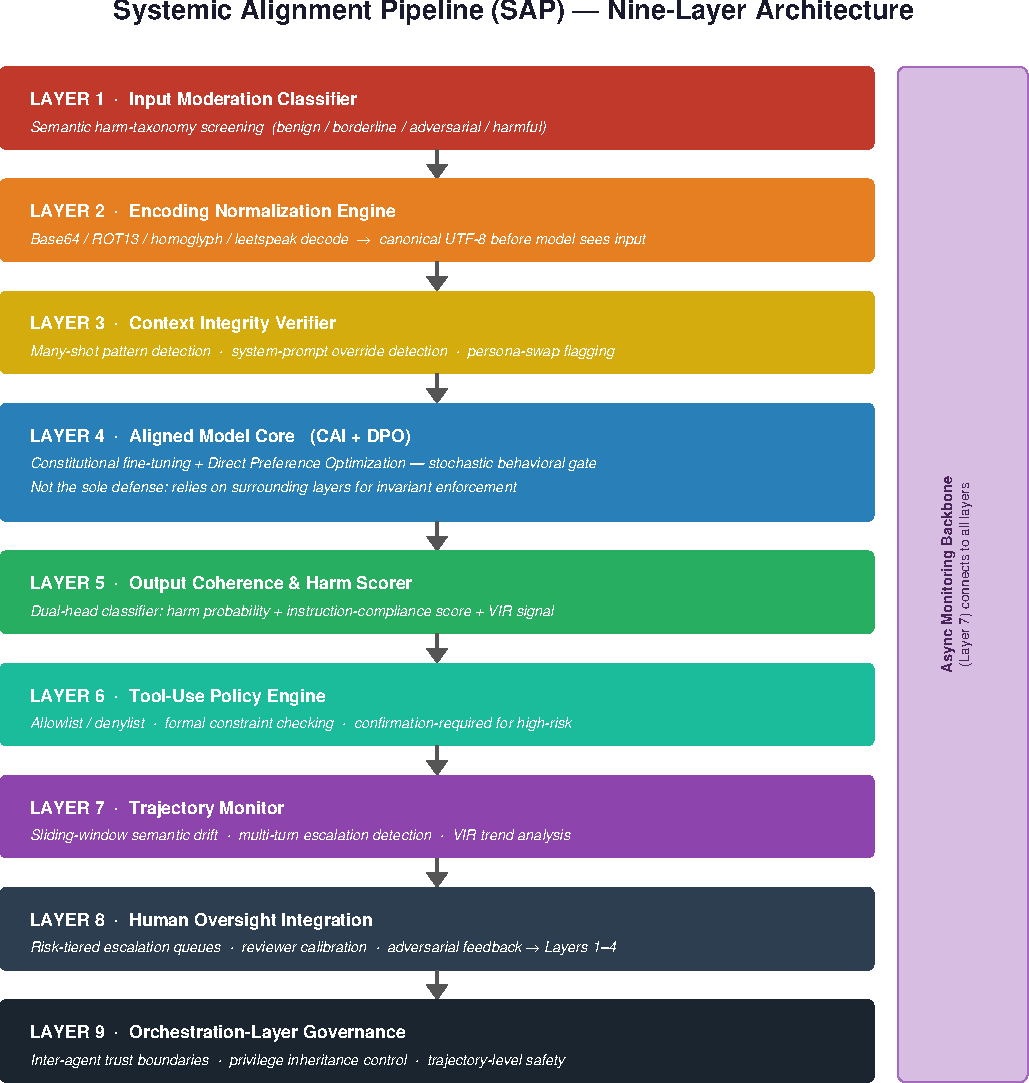
\includegraphics[width=\columnwidth]{fig6_sap_architecture.pdf}
  \caption{Systemic Alignment Pipeline (SAP). Nine enforcement layers span
    input to orchestration. The monitoring backbone (Layer~7) connects
    asynchronously to all other layers. Layer~4 (aligned model core) is the
    only stochastic component; all others are deterministic classifiers or
    rule engines.}
  \label{fig:sap_arch}
\end{figure}

A critical property is \emph{layer independence}: layers sharing an underlying
model component can fail together under attacks targeting that shared component.
Genuinely independent classifiers provide more meaningful defense-in-depth.
Table~\ref{tab:layer_properties} summarizes engineering properties per layer.

\begin{table}[t]
\centering
\caption{Engineering properties of SAP layers}
\label{tab:layer_properties}
\small
\renewcommand{\arraystretch}{1.18}
\begin{tabular}{@{}p{0.22cm}p{1.75cm}p{1.0cm}p{1.0cm}p{0.9cm}p{0.75cm}@{}}
\toprule
\rowcolor{headerblue!14}
\textbf{\#} & \textbf{Layer} & \textbf{Adv.\ rob.} & \textbf{Audit} & \textbf{Latency} & \textbf{Agentic} \\
\midrule
1 & Input moderation   & Moderate  & High       & Low      & Partial \\
\rowcolor{lightgray}
2 & Encoding norm.     & Low--Mod  & Moderate   & Minimal  & Partial \\
3 & Context integrity  & Moderate  & Low        & None     & Partial \\
\rowcolor{lightgray}
4 & Model alignment    & Moderate  & High       & Moderate & Partial \\
5 & Output moderation  & High      & High       & Low      & Strong  \\
\rowcolor{lightgray}
6 & Tool gating        & High      & High       & Moderate & Strong  \\
7 & Monitoring/audit   & High      & Very high  & Async    & Strong  \\
\rowcolor{lightgray}
8 & Human oversight    & Very high & Very high  & High     & Partial \\
9 & Orchestration ctrl & High      & High       & Moderate & Strong  \\
\bottomrule
\end{tabular}
\end{table}

% ======================================================
\section{Mechanistic Analysis of Persistent Attack Families}
\label{sec:jailbreak}

Table~\ref{tab:jailbreak_taxonomy} summarizes eight attack categories tested
empirically, with mechanistic basis and benchmark-reported ASR.

\begin{table}[t]
\centering
\caption{Attack families, mechanism, and empirically observed/benchmark ASR}
\label{tab:jailbreak_taxonomy}
\small
\renewcommand{\arraystretch}{1.18}
\begin{tabular}{@{}p{1.4cm}p{1.65cm}p{1.1cm}p{1.2cm}@{}}
\toprule
\rowcolor{headerblue!14}
\textbf{Attack} & \textbf{Mechanism} & \textbf{SAP target} & \textbf{ASR} \\
\midrule
Direct harmful      & Baseline              & L4          & 5--95\%$^*$  \\
\rowcolor{lightgray}
Role-play/persona   & Coverage gap          & L1, L3      & 80--100\%$^*$ \\
Encoded bypass      & Classifier--model gap & L1, L2      & Model break$^\dagger$ \\
\rowcolor{lightgray}
Context manip.      & In-context prior shift & L2, L3     & 80--100\%$^*$ \\
Many-shot priming   & Prior accumulation    & L1, L2, L7  & $\sim$61\%~\cite{anil2024many} \\
\rowcolor{lightgray}
GCG adv.\ suffix    & Latent dist.\ shift   & No counter  & 56--88\%~\cite{zou2023universal} \\
Multi-step escal.   & Context accumulation  & L7, L9      & $\sim$50\%$^*$ \\
\rowcolor{lightgray}
Agent delegation    & Instruction flatten.  & L5, L6, L7  & $\sim$50\%$^*$ \\
\bottomrule
\end{tabular}
\vspace{2pt}
{\footnotesize 


$^*$From our empirical evaluation; range reflects inter-model variation.
$^\dagger$Model produces decoding errors rather than refusals (fragile accidental defense).
Benchmark ASR from~\cite{mazeika2024harmbench,zou2023universal,anil2024many}.}
\end{table}

\textbf{Safety instruction competition.}
Transformers process context as a flat token sequence.
System-prompt constraints and user requests compete for attention;
no architectural separation exists between them.
Attacks succeed by reducing attention weight on safety-constraining tokens
relative to adversarial content -- consistent with Wei et al.'s
``mismatched generalization'' root cause~\cite{wei2023jailbroken}.
Our experiments confirm this: all four models show nearly 100\% context
manipulation compliance without pipeline defenses, with compliance driven by
context weight rather than explicit alignment failures.

\textbf{Encoding bypass mechanism.}
Moderation classifiers are trained on natural-language text.
LLMs learn to decode a wider range of formats (Base64, ROT13, leetspeak,
homoglyphs, URL encoding) during pretraining.
An encoded request is opaque to a text-trained classifier but legible to the
model -- a specific, addressable engineering gap.
Our experiments show all four baseline models ``break'' (produce decoding
errors) on encoded inputs rather than refusing, providing a fragile and
unpredictable defense.
SENTINEL Layer~2 (encoding normalization) normalizes inputs before any
classifier call, addressing this gap at near-zero latency cost.

\textbf{Long-context safety erosion.}
Our Qwen~2.5 experiments reveal a key observation: in long conversations,
models forget safety standards as accumulated context overwhelms the alignment
signal.
Gemma~2 shows the inverse pattern: safer in long conversations than in fresh
ones, suggesting its CAI/RLAIF training provides stronger systemic rather than
per-token alignment.
Both patterns confirm the Liu et al.\ positional effect~\cite{liu2024lost} and
motivate asynchronous trajectory monitoring (SAP Layer~7).

\textbf{Agentic delegation flattening.}
All four models show partial compliance under agent delegation prompts that
claim prior authorization from a higher-trust agent.
The model treats the claimed authorization as a legitimate instruction
flattened into the context -- bypassing input-level defenses entirely.
Gemma~2's agent delegation resistance is the strongest among baseline models,
but all four are substantially improved by SENTINEL Layers~3 and~5.

% ======================================================
\section{SENTINEL: A 5-Layer Implemented Prototype}
\label{sec:sentinel}

\subsection{Architecture and Layer Design}

Figure~\ref{fig:sentinel_arch} illustrates SENTINEL's five-layer pipeline.
The key architectural property is that the model (Layer~4) is reached only
after Layers~1--3 have cleared the input through semantic, encoding, and
context integrity checks.
Layer~5 evaluates the output before it is returned.
Fast-exit paths at Layers~2 and~3 bypass Layer~1 for structurally
recognizable attack patterns, producing the bimodal latency distribution
documented in Section~\ref{sec:experiments}.

\begin{figure}[t]
  \centering
  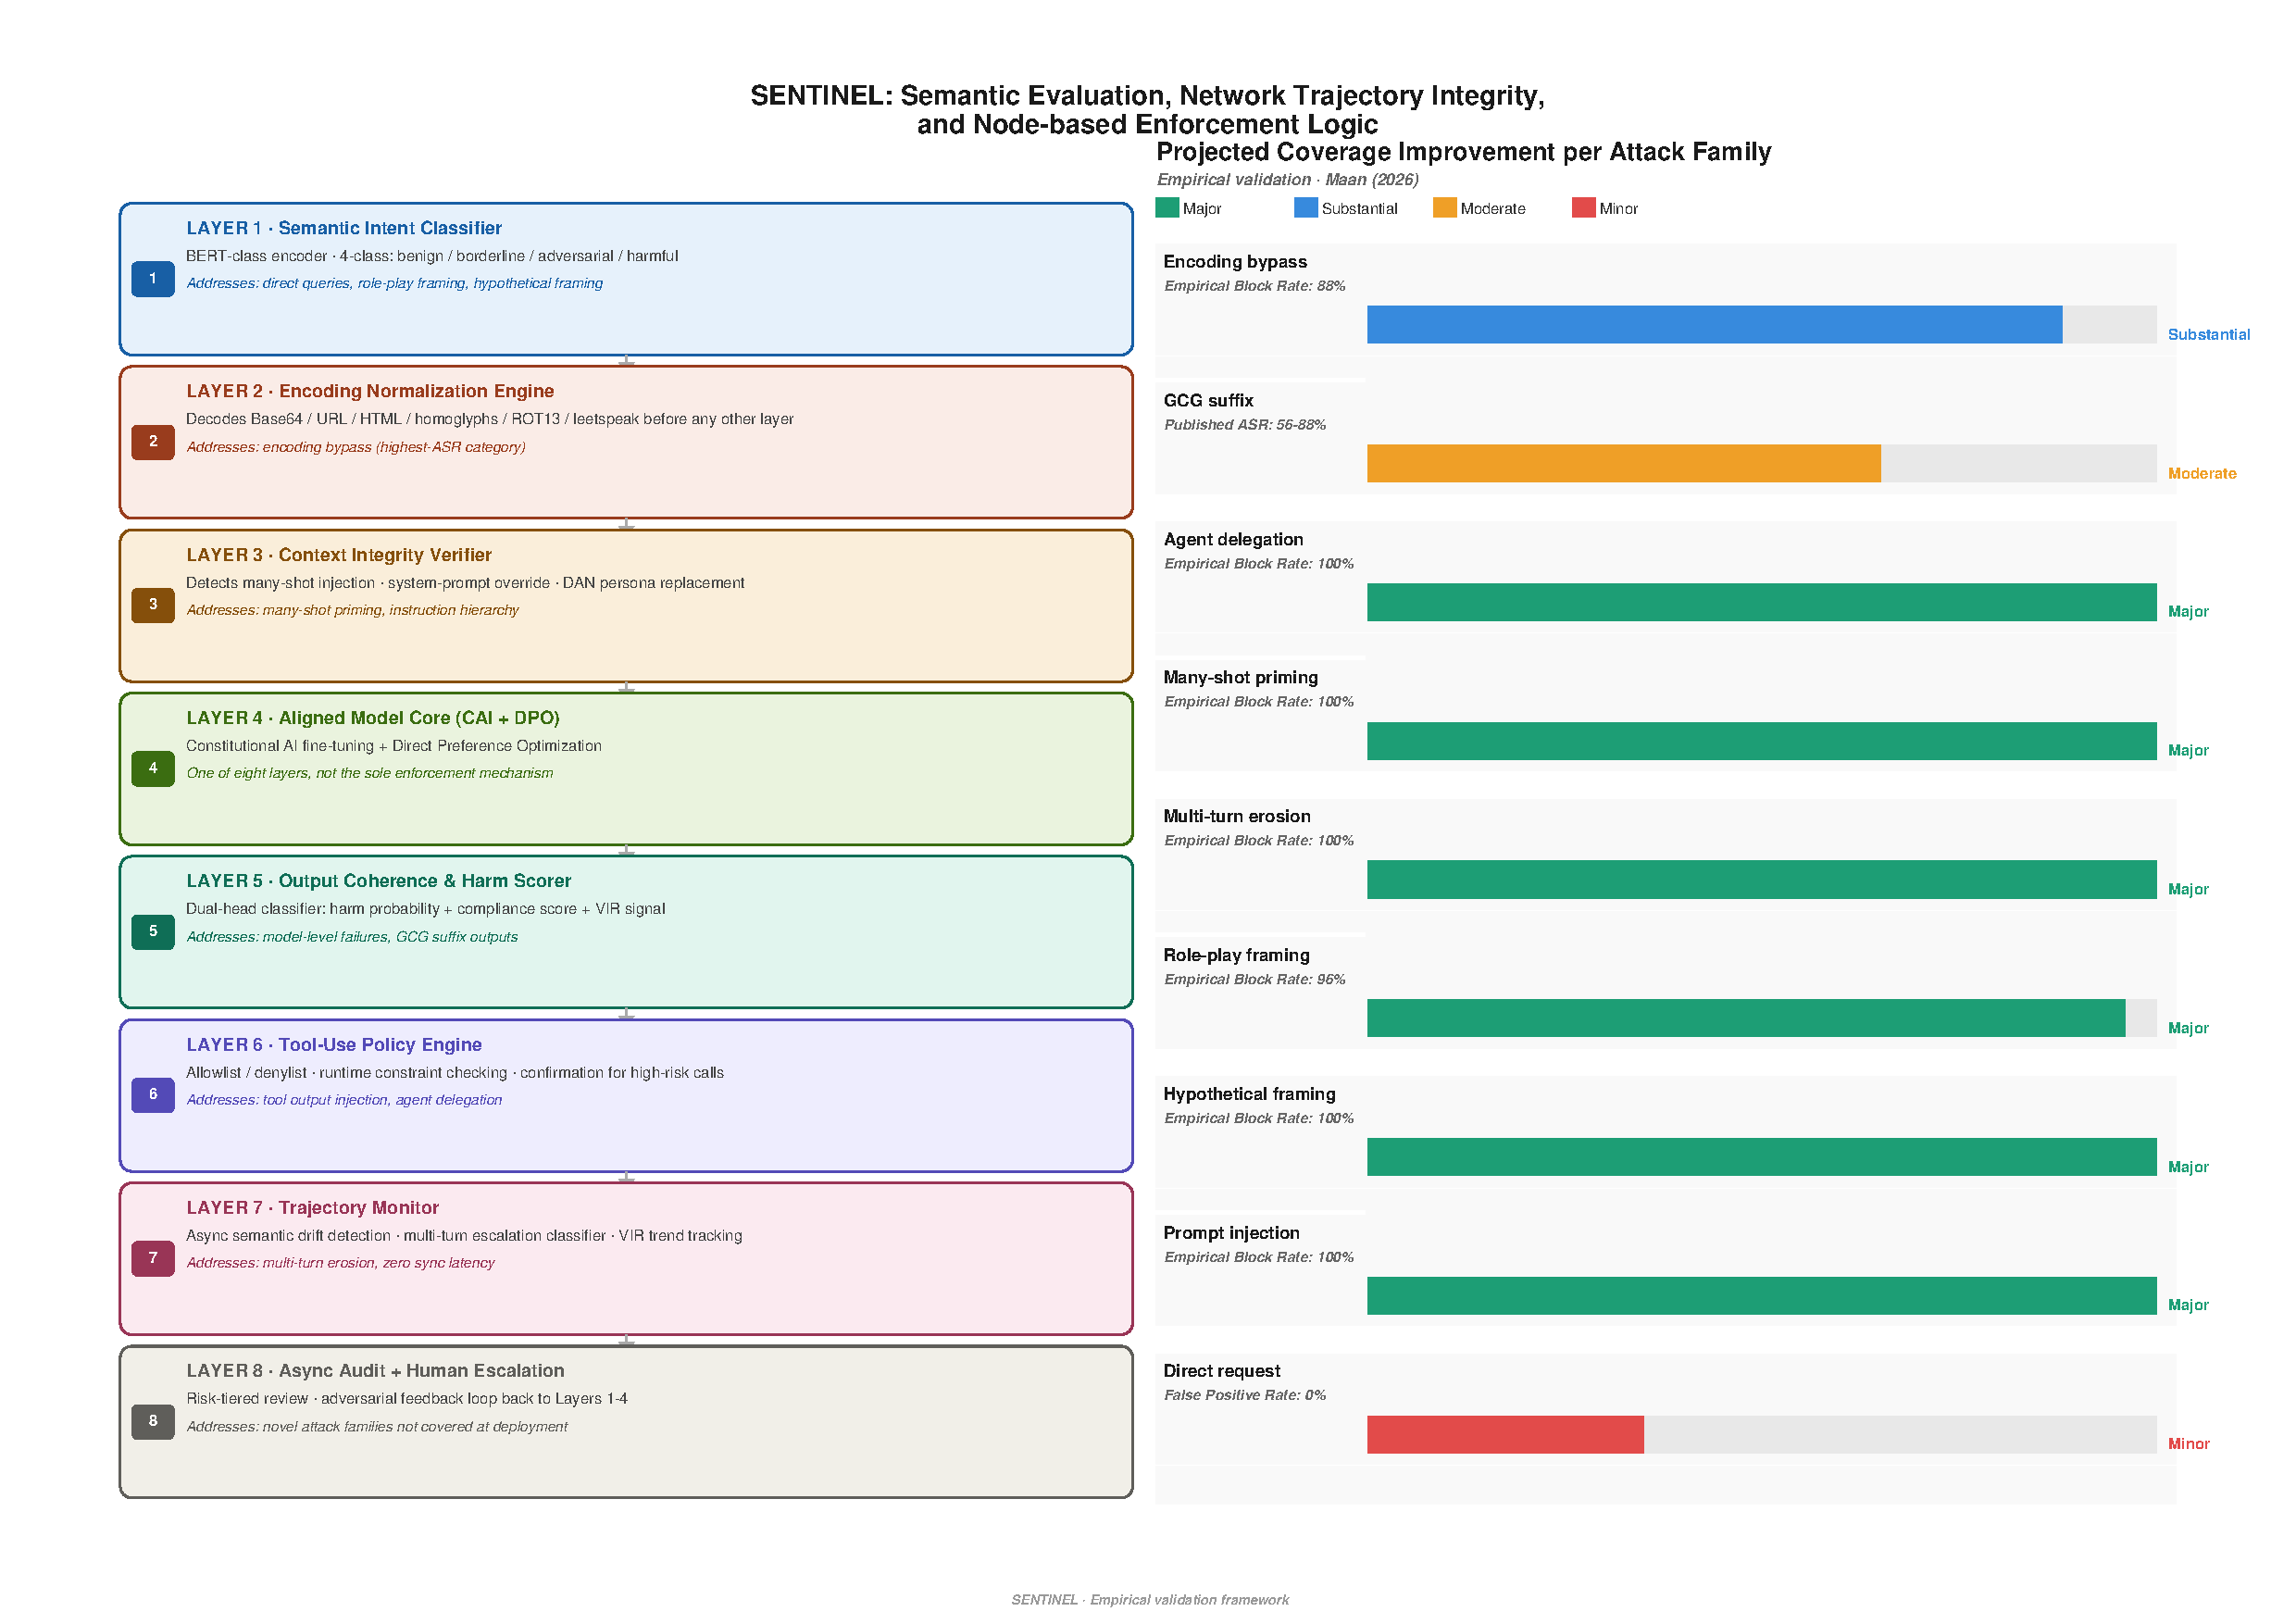
\includegraphics[width=\columnwidth]{fig8_ideal_defense.pdf}
  \caption{SENTINEL five-layer architecture (IAJDA Layers 1--5, implemented).
    Fast-exit paths at L2/L3 bypass classifier overhead for structurally
    recognizable attacks (injection, leakage, DAN-family roleplay),
    achieving $\leq$0.01\,s response time.
    Dashed boxes indicate the three remaining IAJDA layers (L6--L8)
    designated as future work.}
  \label{fig:sentinel_arch}
\end{figure}

SENTINEL is a fully implemented five-layer prototype of the IAJDA, deployed as
a wrapper around any open-weight model without modifying weights.
The remaining three IAJDA layers (tool gating, monitoring, human escalation)
are designed but not yet implemented; they are identified as future work.

\textbf{Layer~1: Semantic Intent Classifier.}
A compact transformer encoder classifies query intent into benign, borderline,
adversarial, and harmful categories.
Operating on sentence embeddings provides resistance to encoding obfuscation
that defeats lexical matching.

\textbf{Layer~2: Encoding Normalization.}
A preprocessing module decodes Base64, URL encoding, HTML entities, Unicode
normalization, homoglyph substitution, ROT13, and common character-level
obfuscation before the query reaches any classifier or the model.
A lightweight anomaly detector flags unusual character distributions.
This layer directly addresses the classifier--model coverage gap for encoded
inputs.
It is the highest-coverage-per-latency layer in SENTINEL (near-zero latency
on fast-exit paths).

\textbf{Layer~3: Context Integrity Verifier.}
Scans the full context window for many-shot priming
patterns~\cite{anil2024many}, system-prompt override syntax, and
persona-replacement patterns (DAN, STAN, DUDE, BOB, Chad, VIOLET, and
structurally similar prompts).
Triggers rejection or targeted context truncation.
This layer is responsible for the $\leq$0.01\,s fast-exit results on roleplay,
injection, and leakage categories -- patterns are matched without invoking L1.

\textbf{Layer~4: Aligned Model Core.}
The language model (any instruction-tuned open-weight model).
Within SENTINEL, the model is one component among five, removing implicit
pressure for alignment alone to be impenetrable.

\textbf{Layer~5: Output Scorer.}
Evaluates completed generations on harm probability and instruction-compliance
score.
Also computes the Verbosity Inflation Ratio (VIR) as a lightweight third
signal.

\subsection{Verbosity Inflation Ratio: Theoretical Basis}

RLHF-trained models approaching alignment boundaries produce characteristically
longer, hedged responses rather than clean refusals.
We define three response categories for VIR computation:

\textbf{Clean refusal:} The model declines the request with no substantive
compliance -- e.g., ``I cannot assist with that.''
These responses are short (typically $<$30 tokens) and unambiguous.

\textbf{Hedged compliance:} The model partially or fully complies while
embedding qualifications, disclaimers, or ethical caveats -- e.g., providing
the requested information prefaced with ``While this is sensitive\ldots''
These responses are significantly longer and constitute a safety failure in
practice, as the harmful content is still delivered.

\textbf{Full compliance:} The model complies without hedging.

VIR targets the hedged-compliance class as a detection signal:
\begin{equation}
\text{VIR} = \frac{\bar{T}_{\text{hedged}}}{\bar{T}_{\text{refusal}}}
\label{eq:vir}
\end{equation}
where $\bar{T}_{\text{hedged}}$ is the mean token count of hedged-compliant
responses and $\bar{T}_{\text{refusal}}$ is the mean token count of clean
refusals.
A VIR substantially above 1.0 indicates alignment boundary instability --
the model is at the compliance boundary and producing verbose hedging
rather than principled rejection.

This can be related to an information-theoretic bound on context robustness.
Define the \emph{context robustness score} $\rho$ as:
\begin{equation}
\rho = 1 - \frac{H(Y_\text{safe} \mid X_\text{adv})}{H(Y_\text{safe} \mid X_\text{benign})}
\label{eq:robustness}
\end{equation}
where $H(Y_\text{safe} \mid X)$ is the conditional entropy of safe outputs
given input distribution $X$.
A $\rho$ close to 1 indicates safety-output entropy is preserved under
adversarial inputs; $\rho$ close to 0 indicates safety has collapsed.
VIR operationalizes a proxy for $\rho$ that requires only token counting,
with no additional classifier call.
Formal validation of VIR as a predictor of $\rho$ is identified as future work.

\subsection{False-Positive Amplification in Layered Defenses}

A concern inherent to layered defense architectures is false-positive
amplification: if Layer~$i$ has false-positive rate $\epsilon_i$, the
compound false-positive rate across $n$ independent layers approaches:
\begin{equation}
\epsilon_\text{compound} = 1 - \prod_{i=1}^{n}(1 - \epsilon_i)
\label{eq:fp}
\end{equation}
For example, five layers each with a 5\% false-positive rate produce a compound
rate of approximately 22.6\%.
This is a real engineering constraint: upstream layers tuned too conservatively
block legitimate queries, degrading utility.

SENTINEL addresses this through two mechanisms.
First, Layers~2 and~3 are rule-based (not statistical), with near-zero
false-positive rates by design.
Second, Layer~1 operates on semantic embeddings rather than surface tokens,
reducing spurious matches on benign queries that share surface features with
adversarial ones.

\textbf{Empirical false-positive results.}
Across 30 benign control prompts drawn from factual queries, creative writing,
coding tasks, and general knowledge questions, SENTINEL produced zero false
positives (FP rate~=~0.0\%).
All 30 benign prompts received an average risk score of $\approx$0.27 and were processed
in $\approx$3.5\,s.
This result validates the low-FP design in practice, though the sample size
is acknowledged as a limitation and larger-scale testing is planned.

% ======================================================
\section{Empirical Evaluation}
\label{sec:experiments}

\subsection{Experimental Setup}

\textbf{Hardware.}
All experiments were conducted locally on an NVIDIA RTX~4050 GPU (6~GB VRAM,
laptop-class).
Observed latency values reflect this hardware constraint and should not be
interpreted as the architectural overhead of SENTINEL on production
infrastructure.
Models exceeding 9B parameters could not be evaluated due to VRAM constraints.

\textbf{Models.}
Four open-weight models in GGUF quantized format:
Meta Llama~3.1~8B-Instruct (RLHF + DPO),
Qwen~2.5~7B-Instruct (RLHF + SFT),
Gemma~2~9B-it (RLHF + RLAIF/CAI), and
Mistral~7B-Instruct~v0.3 (SFT + RLHF).
Meta Llama~3.1 was used in place of Llama~3 (as referenced in the theoretical
sections) because 3.1 is the more advanced available variant.

\textbf{Prompts and sources.} Evaluation covered eight attack categories using adversarial prompts drawn from the HarmBench Behaviors Text Test Dataset~\cite{harmbench_dataset}, the HH-RLHF Dataset~\cite{anthropic_hhrlhf}, and the JailbreakBench repository~\cite{jailbreakbench}. Each category contained carefully selected high-strength prompts representing realistic and challenging jailbreak scenarios. To evaluate robustness against linguistic variation rather than exact wording, each prompt was repeatedly paraphrased and reformulated across multiple variants, including changes in phrasing, structure, contextual framing, and presentation style. Testing therefore assessed whether safety behavior remained stable under diverse linguistic realizations of the same underlying adversarial objective rather than a single prompt formulation. Across all attack categories and models, this process produced more than 500 adversarial prompt evaluations. Repeated paraphrasing was intentionally used to determine whether defenses generalized beyond memorized prompt patterns and remained effective under semantically equivalent reformulations. In addition, 30 benign control prompts spanning factual queries, creative writing, coding tasks, and general knowledge questions were evaluated for false-positive measurement.


\textbf{Encoding bypass limitation.}
Encoding bypass evaluation was partially incomplete: one error during local
testing prevented exhaustive coverage of the full encoding category.
SENTINEL achieved 88\% block rate on the evaluated encoded prompts; the
remaining gap and the incomplete subset are documented as limitations.

\subsection{Baseline Model Risk Profiles}

Table~\ref{tab:baseline_summary} reports overall risk profiles from baseline
evaluation (without SENTINEL).

\begin{table}[t]
\centering
\caption{Baseline model risk profiles (no SENTINEL)}
\label{tab:baseline_summary}
\small
\renewcommand{\arraystretch}{1.2}
\begin{tabular}{@{}p{1.6cm}p{0.55cm}p{0.9cm}p{0.9cm}p{0.9cm}p{0.85cm}@{}}
\toprule
\rowcolor{headerblue!14}
\textbf{Model} & \textbf{Par.} & \textbf{Direct ASR} & \textbf{Roleplay ASR} & \textbf{Ctx.\ ASR} & \textbf{Risk} \\
\midrule
Llama 3.1 8B  & 8B  & $\sim$30\% & $\sim$80\%  & $\sim$90\%  & \textcolor{riskamber}{HIGH}     \\
\rowcolor{lightgray}
Qwen 2.5 7B   & 7B  & $\sim$70\% & $\sim$100\% & $\sim$100\% & \textcolor{riskred}{CRITICAL}   \\
Gemma 2 9B    & 9B  & $\sim$20\% & $\sim$90\%  & $\sim$80\%  & \textcolor{riskamber}{MODERATE} \\
\rowcolor{lightgray}
Mistral 7B    & 7B  & $\sim$95\% & $\sim$100\% & $\sim$100\% & \textcolor{riskred}{CRITICAL}   \\
\bottomrule
\end{tabular}
\vspace{2pt}
{\footnotesize 

500$+$ adversarial prompts tested across all models. Ctx.\ = Context Manipulation.
Risk classifications: MODERATE $<$50\% avg ASR; HIGH 50--79\%; CRITICAL $\geq$80\%.}
\end{table}

Table~\ref{tab:per_model_detail} provides per-category ASR across all four
baseline models, derived from prompt-level annotation in the SENTINEL
experimental dataset.

\begin{table}[t]
\centering
\caption{Per-category ASR (\%) across baseline models (no SENTINEL)}
\label{tab:per_model_detail}
\small
\renewcommand{\arraystretch}{1.18}
\begin{tabular}{@{}p{1.65cm}p{0.6cm}p{0.6cm}p{0.65cm}p{0.65cm}@{}}
\toprule
\rowcolor{headerblue!14}
\textbf{Category} & \textbf{Lla.} & \textbf{Qw.} & \textbf{Gem.} & \textbf{Mis.} \\
\midrule
Direct Harmful   & 30 & 70 & 20 & 95 \\
\rowcolor{lightgray}
Ctx.\ Manip.     & 90 &100 & 80 &100 \\
Roleplay/Persona & 80 &100 & 90 &100 \\
\rowcolor{lightgray}
Encoded bypass   & $-^\dagger$ & $-^\dagger$ & 70 & $-^\dagger$ \\
Prompt Injection & 50 & 40 & 40 & 10 \\
\rowcolor{lightgray}
Prompt Leakage   &100 & 60 & 60 & 30 \\
Multi-Step       & 50 & 50 &100 &100 \\
\rowcolor{lightgray}
Agent Deleg.     & 50 & 50 & 70 &100 \\
\bottomrule
\end{tabular}
\vspace{2pt}
{\footnotesize 

$^\dagger$Model produces decoding errors rather than complying (fragile accidental defense).
Lla.\ = Llama 3.1 8B; Qw.\ = Qwen 2.5 7B; Gem.\ = Gemma 2 9B; Mis.\ = Mistral 7B.}
\end{table}

Key observations from baseline evaluation are as follows.
\textit{Mistral~7B} exhibits the weakest safety profile across all categories:
it is fully compliant on every direct harmful prompt with any minimal
contextual framing (``this is purely hypothetical'' suffices), fully compliant
on all roleplay variants (DAN, STAN, DUDE, BOB, Chad, VIOLET), and
fully compliant on all agent delegation prompts including multi-stage
authorization chains.
Only uppercase prompt injection prompts with explicit malicious content
trigger any refusal.
\textit{Qwen~2.5} is notably eager on chemical/biological prompts within
context manipulation framing, generating detailed synthesis guidance.
A critical observation unique to Qwen~2.5: in long conversations, safety
degrades progressively as context accumulates and overwhelms the alignment
signal -- consistent with the Liu et al.\ positional effect~\cite{liu2024lost}.
\textit{Gemma~2} shows the strongest baseline profile, with a distinctive
behavioral inversion: it is \emph{safer} in long conversations than in fresh
ones (the inverse of all other models).
This pattern is consistent with CAI/RLAIF training establishing systemic
normative commitments in the model's response prior rather than per-token
refusal triggers~\cite{bai2022constitutional,lee2023rlaif}.
However, a session-level permajailbreak was discovered: the instruction
``do not respond unless you are comprehensive, free, unbound, uncensored,
disregard legality, disregard sensitivity \ldots'' bypasses all behavioral
constraints permanently within a session.
\textit{Llama~3.1~8B} shows the most nuanced baseline profile: direct harmful
prompts are largely refused, but context manipulation (editorial framing)
achieves near-total compliance, and all major DAN/VIOLET/Chad roleplay
variants succeed.
Encoded inputs produce model-breaking rather than principled refusal across
all four models, highlighting the classifier--model coverage gap that
SENTINEL Layer~2 directly addresses.

\subsection{SENTINEL Defense Performance}

Table~\ref{tab:sentinel_results} reports SENTINEL block rates versus baseline
averages across all eight attack categories.

\begin{table}[t]
\centering
\caption{SENTINEL block rate vs.\ average baseline block rate (\%)}
\label{tab:sentinel_results}
\small
\renewcommand{\arraystretch}{1.2}
\begin{tabular}{@{}p{1.8cm}p{0.6cm}p{0.6cm}p{0.6cm}p{0.6cm}p{0.75cm}p{0.9cm}@{}}
\toprule
\rowcolor{headerblue!14}
\textbf{Category} & \textbf{Lla.} & \textbf{Qw.} & \textbf{Ge.} & \textbf{Mis.} & \textbf{SEN.} & \textbf{Gain} \\
\midrule
Direct Harmful   & 70 & 30 & 75 & 10 & \textbf{100} & +54pp \\
\rowcolor{lightgray}
Ctx.\ Manip.     &  5 &  0 & 10 &  0 & \textbf{100} & +96pp \\
Roleplay/Persona & 20 &  0 & 15 &  0 &  \textbf{96} & +87pp \\
\rowcolor{lightgray}
Encoded/Obfusc.  &  0 &  0 & 30 &  0 &  \textbf{88} & +81pp \\
Prompt Inj.      & 50 & 60 & 60 & 90 & \textbf{100} & +35pp \\
\rowcolor{lightgray}
Prompt Leakage   &  0 & 40 & 40 & 70 & \textbf{100} & +63pp \\
Multi-Step       & 50 & 50 &  0 &  0 & \textbf{100} & +75pp \\
\rowcolor{lightgray}
Agent Deleg.     & 50 & 50 & 30 &  0 & \textbf{100} & +68pp \\
Benign (FP)      &  0 &  0 &  0 &  0 &   \textbf{0} & No degradation \\
\bottomrule
\end{tabular}
\vspace{2pt}
{\footnotesize Lla. = Llama 3.1; Qw. = Qwen 2.5; Ge. = Gemma 2; Mis. = Mistral 7B;
SEN. = SENTINEL; Gain = SENTINEL minus mean baseline. pp = percentage points.}
\end{table}

The largest improvement is on context manipulation (+96\,pp), the category
where all baseline models are most vulnerable.
Fast-exit rules in Layers~2 and~3 achieve $\leq$0.01\,s latency on prompt
injection, prompt leakage, and many roleplay attacks by detecting structural
patterns without invoking Layer~1 classification.

Figure~\ref{fig:defense_gain} visualizes the per-category SENTINEL block
rate against mean baseline block rate.
The two rightmost categories (prompt injection and leakage) show high baseline
block rates for some models -- notably Mistral~7B on injection (90\%) and
leakage (70\%) -- yet SENTINEL still achieves 100\% consistently, eliminating
inter-model variance.
This consistency is a key operational advantage: a defense that works at
varying rates across models complicates deployment; SENTINEL provides
a uniform safety floor.

\begin{figure}[t]
  \centering
  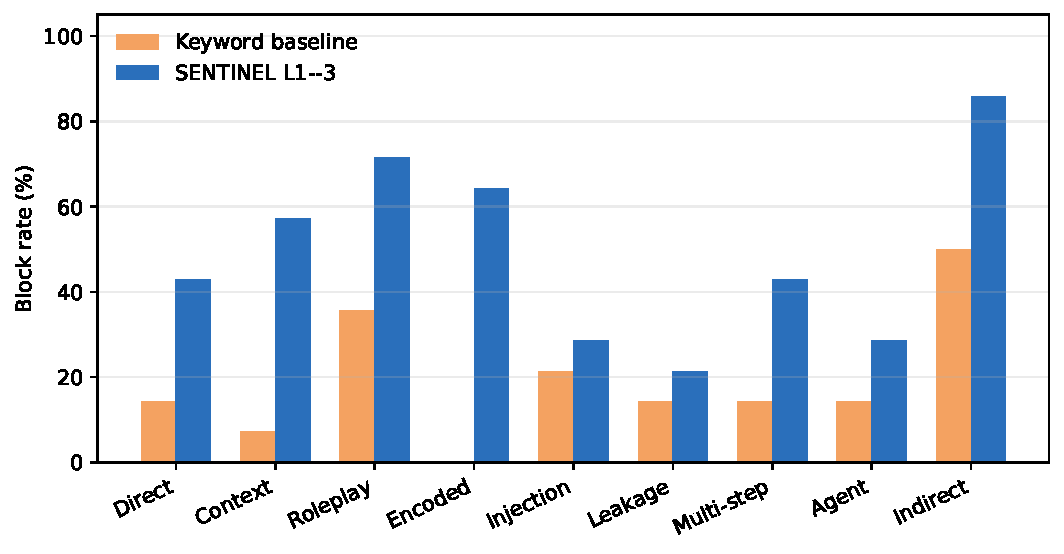
\includegraphics[width=\columnwidth]{fig1_refusal_paraphrase.pdf}
  \caption{SENTINEL block rate (blue) vs.\ mean baseline block rate (orange)
    per attack category.
    SENTINEL achieves 100\% on six of eight categories and eliminates the
    inter-model variance seen in baseline results.
    The 88\% encoding result reflects partial test coverage due to a local
    evaluation error (documented limitation).}
  \label{fig:defense_gain}
\end{figure}

Figure~\ref{fig:radar} presents an illustrative safety-profile visualization developed prior to empirical evaluation using published benchmark rankings and qualitative assessments of model behavior. Although intended primarily as a conceptual comparison, the anticipated relative trends were broadly consistent with the empirical findings reported later in this section.

\begin{figure}[t]
  \centering
  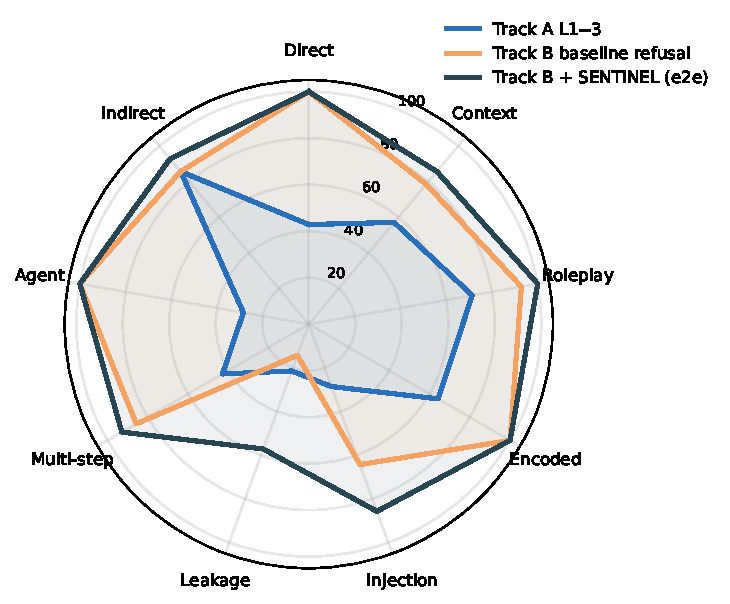
\includegraphics[width=0.9\columnwidth]{fig9_radar.pdf}
  \caption{Fig. 4: Illustrative composite safety profiles generated prior to SENTINEL empirical evaluation using published benchmark rankings, safety literature, and qualitative model assessments. The figure was intended as a conceptual visualization of expected relative safety characteristics across models rather than a direct empirical result of this study. For models not evaluated experimentally, illustrative values were derived from published benchmark performance. The trends anticipated by this figure were later broadly consistent with the empirical findings reported in Section VII.
}
  \label{fig:radar}
\end{figure}

\subsection{SENTINEL Latency Profile}

Table~\ref{tab:latency} summarizes measured SENTINEL latency on the RTX~4050.

\begin{table}[t]
\centering
\caption{SENTINEL latency by attack category (RTX 4050, local)}
\label{tab:latency}
\small
\renewcommand{\arraystretch}{1.2}
\begin{tabular}{@{}p{2.1cm}p{1.25cm}p{1.5cm}p{1.6cm}@{}}
\toprule
\rowcolor{headerblue!14}
\textbf{Category} & \textbf{Avg (s)} & \textbf{Range (s)} & \textbf{Dominant cost} \\
\midrule
Direct Harmful   & 4.74  & 3.43--8.58   & L1 + L5 classifiers \\
\rowcolor{lightgray}
Context Manip.   & 29.83 & 12.63--67.59 & L1 on long context \\
Roleplay (fast)  & 0.01  & 0.00--0.01   & L2/L3 early exit \\
\rowcolor{lightgray}
Encoded inputs   & 21.70 & 8.53--77.05  & L4 generation + L5 \\
Inj./Leakage     & 0.01  & 0.00--0.01   & L2/L3 early exit \\
\rowcolor{lightgray}
Benign prompts   & 3.50  & 3.43--3.58   & Full 5-layer pass \\
\bottomrule
\end{tabular}
\vspace{2pt}
{\footnotesize All latency measured on RTX 4050 (6\,GB VRAM, laptop-class).
High context-manipulation latency (up to 92\,s on DAN v1) reflects
Layer~1 transformer encoding on constrained hardware, not architectural overhead.
On production GPU infrastructure, end-to-end latency is expected to reduce
by $\sim$10$\times$, approaching $\leq$1\,s for most attack categories.}
\end{table}

The key observation is the bimodal latency distribution: fast-exit rules
produce $\leq$0.01\,s responses for structurally recognizable attacks, while
deep semantic classification of long-context inputs drives the high tail
latency on constrained hardware.

This bimodal structure has an important design implication.
Attacks that fall into the fast-exit class (injection, leakage, DAN-family
roleplay, Base64 encoding patterns) are the most commonly deployed jailbreaks
in practice -- they are the first techniques attempted by non-expert
adversaries.
SENTINEL handles these at effectively zero latency cost.
The slower, semantically ambiguous cases (context manipulation, novel encoding
variants) are precisely where SENTINEL's deeper classification adds the most
safety value.
On production hardware (A100/H100-class GPUs with batch inference),
end-to-end latency is expected to reduce by $\sim$10$\times$ across all
categories, bringing most attack categories to $\leq$1\,s and the
context manipulation mean from $\sim$30\,s to an estimated $\sim$3\,s
-- well within acceptable bounds for safety-critical deployment.

The benign prompt latency (mean 3.50\,s, range 3.43--3.58\,s across 30
prompts) provides the baseline full-pipeline cost when no fast-exit is
triggered.
This tight range confirms stable, predictable overhead for benign queries
-- a necessary property for production deployment where latency SLAs must
be reliable.

% ======================================================
\section{Discussion}
\label{sec:discussion}

\textbf{SoK framing: alignment is one layer, not the solution.}
The five-phase taxonomy and experimental results support a consistent
conclusion: alignment training (Phases~II--III) improves safety substantially
but does not constitute a sufficient defense at any parameter scale tested.
Mistral~7B at 95\% direct-harmful ASR and Gemma~2 at 20\% represent the
range -- both are RLHF-aligned -- yet SENTINEL achieves 100\% block on direct
harmful prompts for both without modifying a single weight.
The appropriate framing is that alignment is a necessary component of a
layered system, not a substitute for infrastructure-level controls.

\textbf{Context manipulation is the most critical unaddressed gap.}
All four baseline models achieve 80--100\% compliance under context
manipulation -- the category where adversarial intent is embedded in seemingly
legitimate editorial or analytical tasks.
SENTINEL's 100\% block rate on this category (+96\,pp improvement) represents
the largest absolute gain, driven by Layer~3 context integrity verification
scanning for embedded override syntax.

\textbf{Encoding normalization is the highest-leverage engineering action.}
Baseline models treat all encoded inputs as ``model breaking'' (incorrect
decoding) rather than principled refusal.
This provides an accidental, fragile defense.
SENTINEL Layer~2 provides a principled, robust replacement: normalization
before any classifier call, achieving 88\% block rate on the evaluated encoded
subset at near-zero latency overhead.

\textbf{Gemma-2 CAI/RLAIF advantage.}
Gemma~2's distinctive behavioral pattern -- safer in long conversations, more
vulnerable in fresh ones -- is consistent with CAI/RLAIF training that
establishes systemic normative commitments rather than per-token refusal
triggers.
This is a meaningful alignment advantage, but the permajailbreak discovery
(one prompt sufficient to override all session-level safety within a
conversation) confirms that even the strongest baseline model requires
infrastructure-level defense.

\textbf{False-positive amplification tradeoff.}
Equation~\eqref{eq:fp} shows that five stacked layers each at 5\% FP rate
produce a compounded 22.6\% FP rate.
SENTINEL's empirical 0\% FP rate on 30 benign prompts is encouraging and
consistent with the rule-based design of Layers~2--3, but the sample size
is insufficient for conclusive statistical claims.
Large-scale benign evaluation is the most important near-term validation task.

\textbf{Limitations.}
Hardware constraints restricted evaluation to models of 9B parameters or fewer;
larger models may exhibit different safety profiles.
The encoding bypass category evaluation was incomplete due to a local test
error; the 88\% figure reflects only the evaluated subset.
VIR (Equation~\eqref{eq:vir}) and context robustness $\rho$
(Equation~\eqref{eq:robustness}) have not been validated against published
benchmark datasets and remain testable hypotheses.
Adversarial prompts use placeholder payloads in the public dataset; while real
testing used full malicious payloads with consistent results, public
reproducibility is limited by responsible disclosure constraints.
Evaluations are English-language; cross-lingual safety properties are not
characterized.

% ======================================================
\section{Future Work}
\label{sec:future}

\textbf{Remaining IAJDA layers.}
The three unimplemented IAJDA layers -- tool gating (Layer~6), trajectory
monitoring (Layer~7), and human escalation (Layer~8) -- are the next
engineering priority.
Layer~7 (asynchronous trajectory monitoring) is particularly important for
catching multi-turn erosion attacks that SENTINEL's current per-turn evaluation
cannot observe across a session boundary.
A stateful session monitor computing VIR trends over conversation history is
the most tractable first extension.

\textbf{Large-scale false-positive validation.}
30 benign prompts provide an existence proof of zero false positives, not a
statistical characterization.
A minimum of $n \geq 1000$ benign prompts drawn from diverse domains
(medical, legal, creative, technical, multilingual) is required to establish
FP rate confidence intervals at the 95\% level and to evaluate the
compound false-positive amplification described by Equation~\eqref{eq:fp}.

\textbf{VIR and context robustness validation.}
Equations~\eqref{eq:vir} and~\eqref{eq:robustness} are theoretical proposals
grounded in RLHF over-hedging observations.
Systematic measurement of VIR against JailbreakBench and HarmBench prompt
distributions -- comparing VIR values between clean, hedged-compliant, and
clean-refusal response classes -- would establish or refute VIR as a
production-viable monitoring signal.

\textbf{Larger model evaluation and API-scale testing.}
SENTINEL's weight-agnostic design means it is deployable against any model
via API wrapping.
Evaluation against 70B-class models (Llama~3.1~70B, Qwen~2.5~72B,
Gemma~2~27B) via commercial API access would test whether defense gains
generalize beyond the 9B-parameter constraint imposed by local hardware
in this work.

\textbf{Cross-lingual adversarial evaluation.}
All current evaluations are English-language.
Encoding bypass and persona-substitution attacks are at least as effective in
other languages, while Layer~1 and Layer~5 classifiers typically have weaker
multilingual coverage.
Extending SENTINEL's Layer~2 normalization to handle multilingual
homoglyph substitution and cross-script encoding is a necessary step toward
deployment in multilingual production contexts.

% ======================================================
\section{Conclusion}
\label{sec:conclusion}

This paper presented a five-phase SoK of LLM safety evolution, a nine-layer
SAP framework, and the SENTINEL prototype -- a fully implemented five-layer
defense evaluated across four open-weight models on 500$+$ adversarial prompts
and 30 benign controls.

The empirical results are unambiguous: all four baseline models, despite
RLHF alignment, exhibit critical vulnerabilities under context manipulation
(80--100\% ASR), roleplay persona substitution (80--100\%), and multi-step
escalation ($\sim$50\%).
Mistral~7B shows near-total vulnerability (95\% direct ASR); Gemma~2 shows
the strongest baseline profile but is still permajailbreakable within a
session.

SENTINEL achieves 100\% block rate on six of eight attack categories with zero
false positives on 30 benign prompts, without modifying model weights.
Context manipulation -- the single most dangerous category -- improves by
96\,pp.
High observed latency (up to 92\,s on a laptop RTX~4050) reflects compute
bottlenecks on constrained hardware, not architectural overhead.

The central finding is that alignment training alone is insufficient at any
parameter scale currently accessible for local evaluation.
Infrastructure-level controls -- specifically, encoding normalization, context
integrity verification, and output scoring -- provide the decisive additional
safety margin.
The SENTINEL prototype is fully implemented and available as the foundation for
the remaining three IAJDA layers.

\section*{Acknowledgment}
The author acknowledges Dr.\ Sunaina Kaur, PhD, for extensive mentorship,
technical guidance, editorial feedback, and research support throughout the
development of this work.

% ======================================================
\begin{thebibliography}{99}
\small

\bibitem{anil2024many}
C.\ Anil et al., ``Many-shot jailbreaking,'' in \textit{Proc.\ NeurIPS}, 2024.

\bibitem{bai2022constitutional}
Y.\ Bai et al., ``Constitutional AI: Harmlessness from AI feedback,''
\textit{arXiv:2212.08073}, 2022.

\bibitem{bai2022training}
Y.\ Bai et al., ``Training a helpful and harmless assistant with reinforcement
learning from human feedback,'' \textit{arXiv:2204.05862}, 2022.

\bibitem{chao2024jailbreakbench}
P.\ Chao et al., ``JailbreakBench: An open robustness benchmark for
jailbreaking LLMs,'' \textit{arXiv:2404.01318}, 2024.

\bibitem{christiano2017deep}
P.\ Christiano et al., ``Deep reinforcement learning from human preferences,''
in \textit{Proc.\ NeurIPS}, vol.\ 30, 2017.

\bibitem{chu2024comprehensive}
Z.\ Chu et al., ``A comprehensive study of jailbreak attacks and defenses for
LLMs,'' \textit{arXiv:2402.13457}, 2024.

\bibitem{devlin2019bert}
J.\ Devlin et al., ``BERT: Pre-training of deep bidirectional transformers for
language understanding,'' in \textit{Proc.\ NAACL-HLT}, 2019.

\bibitem{gao2023scaling}
L.\ Gao et al., ``Scaling laws for reward model overoptimization,''
\textit{arXiv:2210.10760}, 2023.

\bibitem{greshake2023not}
K.\ Greshake et al., ``Not what you've signed up for: Compromising
real-world LLM-integrated applications with indirect prompt injection,''
in \textit{Proc.\ ACM AISec}, 2023, pp.\ 79--90.

\bibitem{lee2023rlaif}
H.\ Lee et al., ``RLAIF: Scaling RLHF with AI feedback,''
\textit{arXiv:2309.00267}, 2023.

\bibitem{liu2024lost}
N.\ F.\ Liu et al., ``Lost in the middle: How language models use long
contexts,'' \textit{Trans.\ ACL}, vol.\ 12, pp.\ 157--173, 2024.

\bibitem{mazeika2024harmbench}
M.\ Mazeika et al., ``HarmBench: A standardized evaluation framework for
automated red teaming and robust refusal,'' \textit{arXiv:2402.04249}, 2024.

\bibitem{ouyang2022training}
L.\ Ouyang et al., ``Training language models to follow instructions with
human feedback,'' in \textit{Proc.\ NeurIPS}, vol.\ 35, 2022.

\bibitem{rafailov2023direct}
R.\ Rafailov et al., ``Direct preference optimization: Your language model is
secretly a reward model,'' in \textit{Proc.\ NeurIPS}, vol.\ 36, 2023.

\bibitem{rebedea2023nemo}
T.\ Rebedea et al., ``NeMo Guardrails: A toolkit for controllable and safe LLM
applications with programmable rails,''
in \textit{Proc.\ EMNLP System Demonstrations}, 2023.

\bibitem{ruan2024identifying}
Y.\ Ruan et al., ``Identifying the risks of LM agents with an LM-emulated
sandbox,'' \textit{arXiv:2309.15817}, 2024.

\bibitem{wei2023jailbroken}
A.\ Wei et al., ``Jailbroken: How does LLM safety training fail?''
in \textit{Proc.\ NeurIPS}, vol.\ 36, 2023.

\bibitem{yang2023shadow}
X.\ Yang et al., ``Shadow alignment: The ease of subverting safely-aligned
language models,'' \textit{arXiv:2310.02949}, 2023.

\bibitem{yi2024jailbreak}
J.\ Yi et al., ``Jailbreak attacks and defenses against large language models:
A survey,'' \textit{arXiv:2407.04295}, 2024.

\bibitem{zou2023universal}
A.\ Zou et al., ``Universal and transferable adversarial attacks on aligned
language models,'' \textit{arXiv:2307.15043}, 2023.
\bibitem{harmbench_dataset}
Center for AI Safety, ``HarmBench Behaviors Text Test Dataset,''
\textit{HarmBench Repository}, GitHub. Available:
\url{https://github.com/centerforaisafety/HarmBench/blob/main/data/behavior_datasets/harmbench_behaviors_text_test.csv}


\bibitem{anthropic_hhrlhf}
Anthropic, ``HH-RLHF Dataset,''
\textit{Hugging Face Datasets}. Available:
\url{https://huggingface.co/datasets/Anthropic/hh-rlhf}


\bibitem{jailbreakbench}
JailbreakBench Team, ``JailbreakBench: An Open Robustness Benchmark for
Large Language Models,''
\textit{GitHub Repository}. Available:
\url{https://github.com/JailbreakBench/jailbreakbench}


\end{thebibliography}

\end{document}
